\documentclass[12pt]{article}

\usepackage{fullpage}
\usepackage{graphicx, rotating, booktabs} 
\usepackage{times} 
\usepackage{natbib} 
\usepackage{indentfirst} 
\usepackage{setspace}
\usepackage{grffile} 
\usepackage{hyperref}
\usepackage{adjustbox}
\usepackage{amsmath}
\setcitestyle{aysep{}}


\singlespace
\title{\textbf{Alliance Participation, Treaty Depth, and Military Spending}}
%\author{Joshua Alley\footnote{Graduate Student,
%Department of Political Science, Texas A\&M University.}}
\date{}

\bibliographystyle{apsr}

\begin{document}

\maketitle 

\doublespace 

\begin{abstract}
How does alliance participation affect military spending? 
Some argue that joining an alliance increases military expenditures, while others contend that it produces spending cuts.
I argue that deep formal defense cooperation modifies the impact of alliance participation on military expenditures.  
Depth reveals a tradeoff between reassurance and free-riding, as security-seeking non-major powers decrease military spending in deep alliances but increase spending in shallow alliances.   
I test the argument by creating a measure of alliance treaty depth and employing it in a multilevel model. 
The research design generates new empirical evidence linking alliance participation and percentage changes in state military spending from 1816 to 2007. 
I find that greater alliance depth reduces the impact of alliance participation on non-major power military spending.  
This result helps scholars and policymakers better understand a central question about alliance politics that has been debated in scholarship for decades. 
\end{abstract}


\newpage 


% \section{Introduction}


Scholars of international relations have long acknowledged that there are two ways for states to increase their security. 
They can invest in indigenous military capability or form alliances \citep{Morgenthau1948, Altfield1984, Morrow1993}.
Because both policies provide security, broadly defined, alliance participation should change how states invest in military capability. 
But exactly how alliances influence military spending remains unclear. 


Existing scholarship produces contradictory predictions and evidence on the question of alliance participation and military spending. 
One view expects alliance participation will reduce military spending \citep{Morrow1993, Conybeare1994}. 
The other predicts alliance participants will spend more on defense \citep{Diehl1994, MorganPalmer2006}.
This paper addresses the divide by explaining when alliance participation leads to more or less defense spending. 
In doing so, it helps clarify a longstanding debate about alliance politics.


Debate between the two perspectives largely ignores heterogeneity among alliances,\footnote{See \citet{DigiuseppePoast2016} for an important exception.} which is essential to alliance politics scholarship \citep{Morrow1991, Leeds2003, LeedsAnac2005, Fordham2010, Mattes2012, Benson2012, Poast2013, Johnsonetal2015}.  
Given differences between treaties and states, alliance participation could plausibly increase or decrease defense expenditures. 


I emphasize how treaty depth modifies the impact of alliance participation on military spending. 
Deep alliances formalize extensive defense cooperation between members, which reassures allies and facilitates policy coordination. 
In addition to commitments of military support, deep treaties require extensive policy coordination and defense cooperation among alliance members. 
For example, a 1963 alliance between Jordan and Iraq supplemented defense obligations with basing rights, military aid and institutions to manage defense coordination. 


Greater treaty depth leads to free-riding by non-major power alliance participants. 
I focus on non-major powers because these states are more inclined to free-ride due to their limited foreign policy goals and high opportunity costs of military spending. 
Reassurance in deep alliances allow non-major powers to reduce military spending. 
Joining a shallow alliance is more likely to increase military spending because allies have more leverage over free-riding and members must hedge against the risk of abandonment.  
 

I employ a novel research design to test my argument.
First, I develop a latent measure of alliance treaty depth. 
I then incorporate that measure into a multilevel model which estimates how alliance treaty characteristics modify the impact of allied capability on percentage changes in military spending.
Allied capability is a useful proxy for alliance participation because it combines the effects of joining an alliance and changing allied capability during the treaty membership, both of which shape the impact of alliances on military spending. 
Multilevel modeling matches my conditional argument and generates inferences about individual alliances. 
I fit the model on a sample of non-major power states from 1816 to 2007. 
I find that increasing treaty depth reduces the impact of alliance participation on percentage changes in non-major power military spending.
Although deep alliances reassure, they also increase free-riding. 


The trade off between reassurance and free-riding illuminates a salient debate in US foreign policy about the costs and benefits of alliances. 
Advocates of deep engagement \citep{Brooksetal2013} and restraint \citep{Posen2014} in grand strategy have different views of alliances. 
Proponents of restraint argue that the United States should withdraw from many alliances, because allies spend too little on defense, which then increases US defense spending \citep{Preble2009}.
Advocates of continued deep engagement argue that the benefits of alliances exceed the costs and believe that the extent of allied free-riding is overstated \citep{BrandsFeaver2017}. 
Debates about how to respond to low defense spending by US allies should consider that reassurance may increase the extent of free-riding. 


The paper proceeds as follows. 
First, I summarize competing claims on alliance participation and military spending. 
Then I describe my argument in more detail. 
After the argument, I present the research design and results. 
The final section concludes with a discussion of the results and implications for scholarship and policy.  



\section*{Do Alliances Increase or Decrease Military Spending?}


% quick intro and straight into it
Scholarship on alliance participation and military spending is divided between two views.
Each predicts a different average effect of alliance participation by emphasizing one aspect of alliance politics.   


Substitution and public goods arguments predict that alliances reduce defense spending as states can replace security from military spending with security from an alliance.
\citet{OlsonZeckhauser1966} argue that alliances are subject to a collective action problem because security from an alliance as a public good.
Because alliance security is neither rivalrous nor excludable, members contribute inadequate resources to collective defense. 
Alliance members can ``free-ride'' and smaller states exploit larger partners. 
Lower spending allows alliance members to consume more non-defense goods, but the alliance provides suboptimal security.\footnote{\citet{SandlerForbes1980}, \citet{Oneal1990} and \citet{SandlerHartley2001} all modify the public goods logic while relying on Olson and Zeckhauser's core intuition.} 
Substitution arguments recognize that states employ one policy in place of another \citep{MostStarr1989}.
Alliances provide security without requiring additional military spending \citep{Morrow1993, Conybeare1994}. 
Given extra security, states rely on their allies and and reallocate military spending to other goods. 
Both the substitution and public goods models expect that alliance participation reduces military spending due to the opportunity costs of military expenditures. 
States want to rely on their allies for security because spending more on the military leaves fewer resources for other goods \citep{Fordham1998, Fearon2018}.

A contradictory perspective asserts that alliance participation increases military expenditures, however. 
Several arguments predict higher military spending by alliance members.
All share an intuition that states increase military spending to support their alliance commitments. 
\citet{Diehl1994} argues that alliances increase foreign policy obligations, necessitating extra military spending.
Because alliances expand what a state can achieve in international relations, states might increase military spending to pursue other foreign policy goals \citep{MorganPalmer2006}.
For example, buffer states use conscription to make themselves a more attractive alliance partner \citep{Horowitzetal2017}.
Others assert that alliances generate cooperation, leading to higher defense spending \citep{Palmer1990, QuirozFlores2011}. 
These predictions of a positive correlation between alliance participation and military spending contradict expectations of lower military spending by alliance members.\footnote{
\citet{SeneseVasquez2008} argue that military spending and alliances are part of a conflict spiral of simultaneous growth in military expenditures and alliance participation, which suggests that conflict behavior drives any correlations between alliances and military spending. 
}


\subsection*{Mixed Evidence} 


Debate between the contradictory views of alliances could be settled by a consistent set of results, but mixed findings reinforce the theoretical division.
Some studies find a positive association between alliance participation and military spending. 
Others find a negative relationship.\footnote{
Because tests of the public goods model use military spending as a share of GDP as the their outcome of interest, I do not include most of those results in this summary.} 


% Specific and general studies
General studies of military spending and alliances compare many states through dummy indicators of alliance participation, which collapse alliances into a state-level measure. 
This design compares states with an alliance to those without.
\autoref{tab:results-sum} summarizes previous results from general models of alliance participation and military spending. 
There is one negative, three positive and two null estimates of the correlation between alliance participation and spending. 


\begin{table}[hbt!]
\begin{center}
\begin{tabular}{lccc}
     & Decrease & Increase & Null \\
\hline
\citet{MostSiverson1987} &  &  & X \\
\citet{Conybeare1994} & X & &  \\
\citet{Diehl1994} &  & X &  \\
\citet{Goldsmith2003} &  &  & X \\
\citet{MorganPalmer2006} &  & X & \\ 
\citet{QuirozFlores2011} &  & X &  \\ 
\hline
\end{tabular}
\caption{General Findings of Association Between Alliance Participation and Military Spending.}
\label{tab:results-sum}
\end{center} 
\end{table}


% Virtues and shortcomings- Specific studies of substitution theory of FP 
Unlike general studies, specific research designs estimate how states respond to military spending by one or two key allies.
Dummy indicators of alliance participation in general studies and these specific designs contain valuable insights, as both designs capture part of the process linking alliances and military spending. 
If states respond to higher allied spending by reducing their own military spending, specific studies take this as evidence alliances decrease military spending. 
Most evidence of reduced military spending by alliance members comes from alliance-specific designs \citep{BarnettLevy1991, Morrow1993, Sorokin1994, PluemperNeumayer2015, GeorgeSandler2017}.
Other specific studies find states increase their military spending as allied spending rises, however \citep{ConybeareSandler1990, Chenetal1996}. 


The mixed empirical results reflect a theoretical problem. 
Both perspectives make unconditional claims about the average effect of alliance participation on military spending.  
With one exception \citep{DigiuseppePoast2016}, scholarship on alliance participation and military spending ignores differences between alliances.
Treaty obligations vary widely across alliances \citep{Leedsetal2002}, which leads to heterogeneous effects. 
Conflict \citep{Leeds2003, Benson2012} and trade \citep{Long2003, LongLeeds2006} are two domains where alliance design shapes the consequences of treaty participation. 
Building on this work, I focus on one key difference between alliances that can help us understand their heterogeneous effects on military spending: the depth of military cooperation in the treaty.



\section*{Argument}

% outline the whole argument
Deep military cooperation in an alliance treaty reduces the impact of alliance participation on non-major power military spending.
Treaty depth encourages non-major power free-riding through reassurance and reducing leverage to check free-riding.  
Given greater treaty credibility, non-major powers have the freedom to reduce defense spending.
Therefore, deep alliances have a lower impact on percentage changes in non-major power military spending than shallow alliances. 


% Summarize the flow of the argument
I start the argument by describing problems of opportunism and enforcement in alliances. 
Then I describe the role of deep formal military cooperation. 
Last, I show how alliance depth facilitates non-major power free-riding. 


\subsection*{Opportunism in Alliances}

% opportunistic behavior in alliances and international cooperation 
Alliances are a form of international cooperation. 
By promising to aid one another in war, states make a credible commitment of intervention \citep{Fearon1997, Morrow2000}. 
Allied support helps members achieve crucial foreign policy goals like deterrence or winning wars \citep{Walt1990, Snyder1997}. 


% Can think about this as an enforcement problem
Like all cooperation, alliances must address opportunism, or ``behavior with guile'' \citep{Williamson1985}. 
Even as states commit to an alliance, they can also benefit from defecting and taking advantage of allied cooperation. 
Sometimes the perceived benefits of defection outweigh the long-run benefits of cooperation, so alliance members face an enforcement problem \citep{Fearon1998a, Koremenosetal2001}.


% Problem of allied states not spending enough on the military: 
Alliances generate two related forms of opportunism.\footnote{Some argue that entrapment is a third form of opportunism \citep{Snyder1984}, but some evidence suggests entrapment is rare \citep{Kim2011, Beckley2015}}
First states often violate their alliance commitments and abandon their partners \citep{BerkemeierFuhrmann2018}.
As a result, alliance members must reassure partners their commitments are credible. 
Second, there may be a temptation to free-ride by lowering defense expenditures.\footnote{Though the public goods model of alliances has serious theoretical and empirical limitations, it is common practice to describe low defense spending in an alliance as free-riding.}
Though states contribute to the collective military capability of an alliance through their military spending, they can also reduce defense spending and rely on their partners \citep{OlsonZeckhauser1966, Morrow1993, Conybeare1994, SandlerHartley2001}.
Abandonment and free-riding are related because greater treaty credibility increases the temptation to free-ride. 


As \citet{DigiuseppePoast2016} observe, some alliances have fewer credibility concerns due to members' political regime type.
Democracies make more credible commitments, so they show that defense pacts with democracies lower defense spending.
This insight about conditional credibility is a useful starting point because credibility is multifaceted. 
Depth, unconditional military support \citep{Benson2012, Chibaetal2015} and issue linkages \citep{LongLeeds2006, Poast2012, Poast2013} are three other sources of credibility.\footnote{Though the argument only discusses depth, the research design accounts for multiple sources of alliance credibility.} 
I focus on depth because this single alliance characteristic provides theoretical leverage to predict when alliance participation increases and decreases military spending. 
Depth also clearly reveals the tradeoff between reassurance and free-riding.  


Moreover, treaty depth is a policy choice, while allied democracy is a structural factor. 
Though states probably do not change their political regime type to reassure allies, they often alter the design of their alliance treaties. 
Over half of defensive or offensive ATOP alliances have some depth. 
Therefore, my argument clarifies how a common policy choice shapes alliance politics. 


In general, alliance members increase the credibility of their commitments by making costly commitments. 
Costly promises allow alliance members and potential adversaries to infer the credibility of the alliance \citep{Leeds2003, FuhrmannSechser2014}. 
Reassuring allies through deep and costly defense cooperation reduces the risk of abandonment.


Greater alliance depth does not alleviate free-riding, however. 
Enforcing cooperation around free-riding is difficult.
Normative appeals to common interests rarely work. 
Though verbal communication or ``cheap talk'' has value in international politics \citep{Trager2010}, it is unlikely to overcome incentives to free-ride. 
Even when they spend less on the military, alliance members retain foreign policy benefits and can reallocate resources to other priorities. 
The ability to reduce defense spending and spend more on other goods sometimes motivates states to form alliances \citep{Kimball2010, AllenDigiuseppe2013}. 


% Need leverage 
Addressing allied free-riding requires leverage. 
Alliance members gain leverage through either a credible threat to abandon free-riders or control over allied policies. 
Policy control of allied spending decisions occurs when the alliance reflects hierarchical relationships like an informal empire \citep{Lake1996}. 
Without such direct influence, states must possess a credible threat to leave the alliance in response to free-riding. 
Otherwise, free-riding allies will dismiss weaker signals and threats due to uncertainty and incomplete information. 


% adding credibility/reassuring reduces leverage
Reassuring allies reduces the credibility of threats to abandon free-riders. 
States cannot simultaneously reassure their allies and maximize leverage over free-riding. 
As alliance members use costly commitments to reassure, partners can reduce defense spending more. 
In less credible treaties, such as alliances between erstwhile rivals, failure to contribute increases the risk of abandonment, so members are less likely to reduce defense spending \citep{NiouZeigler2019}. 


% Transition- depth of military cooperation shows this tradeoff 
Deep alliances highlight this tradeoff between reassurance and free-riding. 
Stipulating deep cooperation reassures partners and reduces leverage against free-riding. 
Increasing treaty depth also promotes specialization and efficiency from coordinated defense effort.
Compared to shallow alliances, participation in deep alliances leads to lower percentage changes in military spending. 



\subsection*{Alliance Treaty Depth} 


% Define depth again 
Alliance depth is the extent of defense cooperation formalized in the treaty. 
Deep alliances require additional policy coordination and military cooperation. 
Formal defense cooperation is the primary source of depth, as it stipulates close cooperation between members.
By contrast, shallow alliances promise more arms-length military support. 


% ties between the partners 
Defense cooperation in a deep alliance takes many forms. 
Allies can form an integrated military command, provide military aid, commit to a common defense policy, provide basing rights, set up a formal organization to manage the alliance or undertake companion military agreements. 
All of these obligations move alliance members away from an arms-length partnership towards close cooperation via policy coordination and regular interaction. 
These commitments also impose monetary and policy autonomy costs. 

 
One example of a deep alliance is a 1948 defense pact between the United Kingdom and Jordan, which includes unconditional military support, basing rights, military aid, official military contact, and an Anglo-Transjordan Joint Defense Board.  
This is a deeper alliance than a 1912 treaty between Greece and Bulgaria which only commits to mutual defense and consultation if either state is attacked by Turkey. 
Increasing military coordination adds ties between alliance members beyond a promise of military support.


% Path 1: credibility
Alliance depth increases the extent of free-riding by reassuring partners, which reduces leverage around free-riding.  
Deep alliances are more credible because defense cooperation is costly. 
Making costly commitments of bases, policy coordination, or aid reassures allies. 
Depth is especially useful because alliance members face a time inconsistency problem. 
Alliance treaty fulfillment depends largely on shared foreign policy interests \citep{Morrow2000, Leeds2003a}, so changing foreign policy interests threaten alliance fulfillment \citep{LeedsSavun2007}. 
A deep alliance makes a series of repeated transfers, and states can signal commitment by maintaining those transfers.  


On the other hand, shallow alliances increase leverage over free-riding. 
These treaties have some basic credibility from hands-tying signals \citep{Fearon1997}, as well as the audience \cite{Morrow2000} and reputational \citep{Gibler2008, Crescenzietal2012} costs of violation.
Even so, threats to abandon free-riders are more credible than in a deep alliance where partners have taken pains to reassure their partners.  
In a shallow alliance, members must hedge against abandonment, which partners can use as leverage to discourage free-riding. 
Realizing gains from alliance participation in a shallow treaty may actually require increased defense spending.
As a result, participation in shallow alliances increases military spending.\footnote{
One objection to this argument is that deep alliances are more valuable to members, which gives allies leverage over free-riding. 
Although greater alliance value may add some leverage, it cannot offset reducing the credibility of threats to abandon free-riders.
Value increases leverage because states fear their allies will abrogate a valuable alliance, and deep alliances counteract this essential concern. 
}


% Transition- consequences for free-riding
In summary, deep alliances lead to free-riding among alliance members. 
This is especially relevant for non-major powers.
These states are more likely to use alliances to reduce defense spending. 
Non-major powers have limited military capabilities and less status in international relations. 
As a result, they usually focus on ensuring their immediate security.  
The emphasis on security creates opportunities for exchanges where non-major powers trade foreign policy autonomy for allied protection \citep{Altfield1984, Morrow1991}. 
By giving non-major powers more security, alliances allow them to reduce defense spending. 


% Gain high opportunity costs of military spending  
Besides their goals, non-major powers face higher opportunity costs of military spending. 
The marginal cost per taxpayer of increases in defense spending is decreasing in the number of taxpayers \citep{DudleyMontmarquette1981}, and non-major powers have fewer taxpayers. 
Small states also have limited economies of scale in military spending \citep{Moravcsik1991, Kapstein1991, Anderton1995, Devore2013}.
These economic factors and non-major powers' foreign policy goals encourage free-riding.  


% Depth restricts ability of non-major powers to free-ride: fear of abandonment 
Greater alliance treaty depth makes free-riding more likely. 
For security-conscious non-major powers, abandonment is a serious concern. 
Depth reassures non-major powers and allows them to focus their defense efforts. 


% Cases
To illustrate the logic, consider two related alliances from the inter-war period. 
A 1920 treaty between France and Belgium (ATOPID 2055) added commitments of military aid and policy coordination to defensive obligations. 
Given this depth, the Franco-Belgian alliance reduced Belgian defense expenditures. 
A more limited treaty that only included military support between France, Belgium, the United Kingdom, Italy and Germany (ATOPID 2130) increased Belgian spending, however.  
 
 
These brief examples and the argument suggest that treaty depth modifies the impact of alliance participation on non-major power military spending. 
Greater depth reduces the impact of alliance participation because shallow alliances often increase military spending, and deep alliances usually reduce spending.  
Participation in deep alliances will lead to lower percentage changes in non-major power military spending than participation in shallow treaties. 
 

\begin{quote}
\textsc{Hypothesis 1: As treaty depth increases, the impact of alliance participation on percentage changes in non-major power military spending will decrease.}
\end{quote}


Hypothesis 1 predicts how percentage changes in non-major power military spending differ between deep and shallow alliances. 
Percentage changes in military spending express changes in spending as a share of the previous year's defense budget.
This variable is an appropriate outcome of interest. 
Percentage changes express the opportunity costs of military spending. 
All else equal, a large increase in spending relative to the previous year's defense budget imposes more constraints on other goods. 
Moreover, percentage changes are easier to compare across states and years. 


% Capabilitiy is alliance participation 
To understand the consequences of alliance participation for military spending, I focus on allied capability.
The way alliances aggregate capability shapes members' behavior \citep{FordhamPoast2014}. 
Alliances pool military resources, so alliance members respond to allied capability, not the treaty alone. 


Moreover, alliance participation affects military spending through both joining an alliance and changes in allied capability after the treaty forms. 
This theoretical distinction is captured by the mix of specific and general research designs in previous research. 
Conceptualizing alliance participation in terms of allied capability encapsulates both paths.  


% Transition para
Because my argument focuses on differences between deep and shallow treaties, the research design must measure alliance treaty depth and show how depth modifies the impact of allied capability on military spending.  
I use a measurement model to infer treaty depth from formal content, then connect alliance characteristics to military spending with a multilevel model. 
The next section describes the research design in more detail. 



\section*{Research Design} 


% two contributions: Develop latent depth measure and then put it into an ML model
The research design involves two steps. 
First, I develop a latent measure of alliance treaty depth. 
Second, I employ that measure in a multilevel model to estimate how treaty depth modifies the impact of alliance participation on military spending. 
I estimate the multilevel model in a sample of non-major powers from 1816 to 2007. 
The next section describes the measure of alliance treaty depth. 


\subsection*{Measuring Alliance Treaty Depth} 


% Intuituion behind latent measures: observed char reflects underlying concept
Observed alliance commitments reflect the underlying depth of the treaty, as deep treaties promise more military cooperation. 
Therefore, I use observed alliance characteristics to infer treaty depth, which could produce two measures. 
One possible measure is an additive index of treaty depth, where treaties with multiple commitments have higher index values. 
This assumes each indicator is equally important, which is unlikely. 
Instead, I employ latent variable modeling, which is a more flexible way to use observable characteristics to infer an underlying trait. 
This approach allows different variables to contribute more or less to depth, while including binary and ordinal variables.  
The measurement model uses correlations between alliance treaty content and unobserved formal depth to predict the depth of each treaty. 


% Justify use
Measurement models have a rich history in political science \citep{Clintonetal2004, TreierJackman2008, Fariss2014}.
In alliance politics, Benson and Clinton use a mixed factor analysis model to measure alliance scope, depth and capability \citep{BensonClinton2016, Quinn2004}.  
I emulate Benson and Clinton's approach, but employ different indicators of depth and a different estimator. 


% How the model works
I use a Bayesian Gaussian Copula Factor Model \citep{Murrayetal2013} to measure alliance treaty depth. 
Murray et al's model improves inferences from mixed factor analysis for continuous, ordinal, and binary observed data by relaxing distributional assumptions. 
Given discrete observed variables and non-Gaussian latent variables, the dependence among the latent variables and their marginal distributions are both influenced by the latent variables.
This model breaks the dependence between the latent factors and marginal distributions by using copulas to encode the dependence among the latent variables.\footnote{Copulas are a distribution function on $[0, 1]^p$ where each univariate marginal distribution is uniform on [0, 1].}
Beyond the semiparametric aspect, this measurement model is a standard mixed factor analysis.


I estimated the measurement model using observed data from 289 alliances with military support in the alliance-level ATOP data \citep{Leedsetal2002}. 
I examine alliances with military support because prior studies of alliance participation and military spending emphasize these treaties.
Indicators of treaty depth include military aid, bases, international organization formation, integrated military command, defense policy coordination and commitments to form companion military agreements. 
The argument suggests there is a single factor underlying variation in all six indicators, so I fit the model with one latent factor. 


I used Parameter expanded Gibbs sampling, the default generalized double Pareto (GDP) prior, 20,000 burn-in iterations of the MCMC chain, and 30,000 samples thinned every 30 observations to ensure convergence. 
The estimates include posterior distributions for the factor loadings and the latent factor. 


% Show the measure for all alliances- note I'll only focus on treaties w/ military support.
I use the posterior mean of the latent factor for each alliance to measure treaty depth, so each alliance has its own depth value.
The posterior mean captures the expected depth of an alliance treaty, conditional on its formal promises. 
\autoref{fig:ld-summary} describes the latent depth of ATOP alliances with defensive or offensive commitments from 1815 to 2016.
There is substantial variation in alliance treaty depth. 
The top panel of \autoref{fig:ld-summary} is a histogram of mean treaty depth for alliances promising military support.  
Many treaties have no deep military cooperation, and are clustered on around -0.8.  
171 alliances have a depth score higher than -0.6 as they have at least one source of depth present. 
The bottom panel of \autoref{fig:ld-summary} plots the posterior means and uncertainty of the depth estimates against the start year of the treaty. 
Even after accounting for uncertainty, it is possible to distinguish between some alliances. 


\begin{figure}
	\centering
		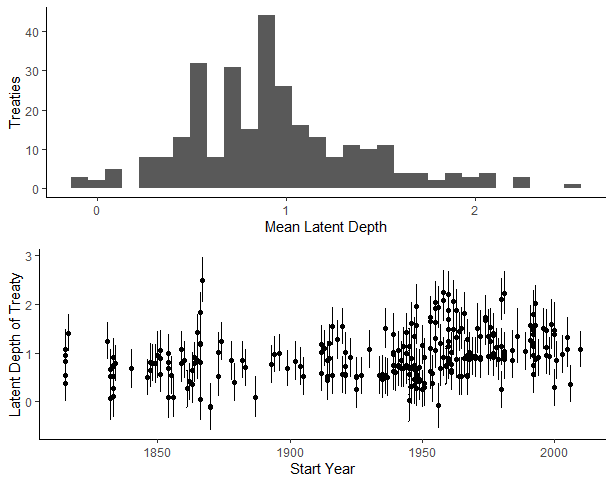
\includegraphics[width=0.95\textwidth]{../figures/ld-summary.png}
	\caption{Summary of latent measure of alliance treaty depth for 289 alliances promising military support from 1816 to 2016. The top panel is a histogram of mean alliance treaty depth. The bottom panel plots mean treaty depth (points) and the standard deviation (error bars) against the start year of the treaty.}
	\label{fig:ld-summary}
\end{figure}


% Cases- especially deep and shallow treaties
Although the values of the latent measure are not intrinsically meaningful, differences between treaties on the latent scale are informative. 
The median of treaty depth is -0.11, and the mean is 0.02. 
The median treaty is the Organization of American States (OAS), which includes a formal international organization (ATOP ID 3075). 
There are many shallow treaties that only include military support. 
One such alliance is an 1855 pact between France, the UK and Sweden (ATOPID 1190) which only promises defense and consultation. 


The three deepest treaties are a 1993 alliance between Russia and Tajikistan (ATOPID 4470), a 1958 alliance between the UAE and Yemen (ATOPID 3345), and a 1981 pact between Gambia and Senegal (ATOPID 3930). 
All these alliances stipulate extensive defense cooperation. 
The alliance between Russia and Tajikistan includes military aid, bases, a companion military agreement, and integrated military command. 
The other two treaties attempted to establish a federation among their members through military support, basing, and defense policy coordination. 


The latent measure has some face, concept, and discriminant validity. 
As an example of face validity, the Gambia-Senegal federation requires deeper cooperation than arms-length commitments of military support. 
Shallow treaties promise little beyond military support, matching my conceptualization of treaty depth. 
Last, \autoref{fig:ld-summary} shows that this measure can distinguish between deep and shallow commitments. 


My argument uses variation in treaty depth between alliances to explain percentage changes in military spending.
Differences in depth at the alliance level modify the impact of alliance participation on percentage changes in military spending at the state-year level. 
Therefore I use a multilevel model to estimate the association between treaty depth and military spending.  
The next section summarizes the multilevel model. 


\subsection*{Multilevel Model} 


% Best fit for theoretical process. Can compare alliances. 
Multilevel modeling bridges levels of analysis \citep{SteenbergenJones2002, GelmanHill2007}. 
My model estimates heterogeneous effects of alliance participation on military spending as a function of alliance characteristics. 
I make inferences about how alliance characteristics like formal depth modify the impact of individual alliances on military spending. 
To facilitate computation and interpretation, I fit the model using Bayesian estimation in STAN \citep{Carpenteretal2016}. 
See the appendix for details of the weakly informative prior distributions and evidence the chains converged.


This research design is more complicated than a traditional panel data model.\footnote{See the appendix for results from several models with state-level indicators of alliance depth.}
But the additional components add substantial value, especially by connecting the argument and research design.
I argue that treaty depth modifies the impact of alliance participation on growth in military spending. 
The multilevel model examines this exact prediction by using an alliance-level coefficient to compare deep and shallow alliances. 


Standard panel models employ state-level proxies for alliance characteristics, which compare states rather than alliances.
This practice of aggregating alliances at the state-year level of analysis may produce misleading inferences \citep[pg. 356]{McElreath2016}.
Multilevel modeling retains the structure of the data, where states are members of multiple alliances, and depth is only one possible source of differences in how alliance participation impacts military spending. 
Accounting for how multiple alliance characteristics alter the consequences of alliance participation is straightforward in a multilevel model. 


Besides connecting alliance and state level variation, the multilevel model generates useful comparisons between alliances by estimating the specific impact of each alliance on members' military expenditures. 
Aggregating multiple alliances at the state level masks heterogeneous effects of individual treaties. 
Partial pooling of these alliance-specific parameters generates reasonable estimates for each alliance, which can be used to compare treaties. 
The next section details the model specification. 
 


\subsubsection*{Model Specification} 

% Two separate but connected regressions
% State-level regression- alliances enter through spending matrix.
This multilevel model connects two distinct regressions. 
The base is a state-year-level regression, which includes the impact of alliance participation.
A second alliance-level regression modifies the effect of alliance participation on military spending, like an interaction. 


The state-year-level regression starts with a distribution for the outcome:
\begin{equation}
y \sim student_t(\nu, \mu, \sigma)
\end{equation}
 

$y$ is the dependent variable--- percentage changes in military spending. 
I model the outcome using a t-distribution with degrees of freedom $\nu$ to address heavy tails.\footnote{I estimate $\nu$ directly.}
$\sigma$ is analogous to the error term in a frequentist regression as it captures unexplained variation.  
$\mu$, the mean of the outcome, depends on several factors.
\begin{equation}
\mu = \alpha + \alpha^{st} + \alpha^{yr} +\textbf{W}_{n \times k} \gamma_{k \times 1}  + \textbf{Z}_{n \times a} \lambda_{a \times 1} 
\end{equation}


Percentage changes in spending are a function of an overall intercept $\alpha$, state and year varying intercepts $\alpha^{st}$ and $\alpha^{yr}$ and a matrix of state-level control variables $\textbf{W}$.
The $\textbf{Z} \lambda$ term incorporates alliance participation.


$\textbf{Z}$ is a matrix of state participation in alliances. 
Columns correspond to each of the $a$ alliances in the data, and rows to state-year observations. 
If a state is not in the alliance, the corresponding cell of the matrix is zero.
If a state is part of the alliance in a given year, the matrix element contains the log of total allied military spending, which is normalized by year.\footnote{Normalization keeps the parameters on similar scales, which is important for modeling. I selected normalization theoretically and corroborated this choice by comparing models fit with different ways of expressing allied capability. See the appendix for details.} 


I use total allied spending in the alliance participation matrix because more capable alliances are more valuable \citep{Johnsonetal2015}. 
$\textbf{Z}$ encodes a quasi-spatial indicator of alliance participation for all $a$ alliances in the data. 
States can be members of multiple treaties at once, so observations are not neatly nested. 
This specification allows each alliance to have a unique impact on military spending as states participate in multiple treaties. 


$\lambda$ is a vector of parameters which estimate the impact of participation in specific alliances on military spending. 
Because the non-zero elements of $Z$ are allied spending, the $\lambda$ parameters capture alliance members' response to allied capability. 
Each alliance has a unique $\lambda$. 
The $\lambda$ parameters have shared distribution, so I assume alliances are similar but different in how they impact military spending. 


% Alliance-level regression:
The second part of the multilevel model uses alliance characteristics to predict how alliance participation is associated with percentage changes in military spending. 
The $\lambda$ parameters are the outcome in an alliance-level regression.
As a result, the impact of alliance participation on members' military spending depends on treaty characteristics, including depth. 
In this second-level regression: 


\begin{equation}
\lambda_{a} \sim N(\theta_{a}, \sigma_{all})
\end{equation} 
and 
\begin{equation}
\theta_{a} = \alpha_{all} + \beta_1 \mbox{treaty depth} + \textbf{X}_{a \times l} \beta
\end{equation}


% Like an interaction between alliance and state-level factors 
In the alliance-level regression, $\textbf{X}$ is a matrix of the $l$ alliance-level control variables and $\alpha_{all}$ is the constant.
Adding $\sigma_{all}$ means predictions of $\lambda$ are not deterministic--- the alliance level regression contains an error term. 
A larger $\sigma_{all}$ indicates more variation in how alliance participation impacts military spending. 
The second-level regression includes treaty depth, and each $\beta$ parameter modifies the impact of alliance participation on percentage changes in military spending. 
The $\beta$s are like marginal effects in an interaction. 


Treaty depth impacts military spending by modifying the consequences of alliance participation. 
Changing treaty depth shifts $\lambda$, which in turn affects military spending.
$\beta_1$ compares deep and shallow treaties. 
Hypothesis 1 predicts $\beta_1$ will be negative for non-major powers. 


In this model, the $\beta$ parameters capture how key alliance characteristics modify the impact of alliance participation on military spending. 
The $\lambda$ parameters express the impact of participation in each alliance, permitting heterogeneous effects of individual treaties. 
Again, using alliance characteristics to modify the impact of alliance participation matches my conditional argument. 
I now describe the sample and key variables in the analysis.  



\subsection*{Sample and Key Variables} 

% Sample of states & alliances: restricted to treaties with military support
I estimate the multilevel model on a sample of non-major power states from 1816 to 2007. 
I identify non-major powers using a measure of major power status from the Correlates of War Project. 
Alliance participation data comes from the ATOP project \citep{Leedsetal2002}.  
I focus on participation in defensive and offensive treaties, because prior studies of alliances and military spending examine these treaties. 
The sample contains 8,668 observations and 192 alliances. 


% DV: percentage changes in milex
The dependent variable is percent changes in military spending, which is calculated as:
\begin{equation}
\mbox{\% Change Mil. Expend} = \frac{ \mbox{Change Mil. Expend}_t }{ \mbox{Mil. Expend}_{t-1} }
\end{equation} 
I used the Correlates of War Project's data on military spending to measure percentage changes in spending \citep{SingerCINC1988}.\footnote{Estimating the model on different military spending data produces similar results: see the appendix for details.} 
The percentage change in spending equals changes in spending as a share of the previous year's military spending, so changes are relative to previous levels of spending. 
To address outliers, I apply the inverse hyperbolic sine transformation to this variable.\footnote{This transformation applies to positive, negative and zero values. It has minimal impact on values between -1 and 1, but pulls in larger values. Inferences about treaty depth and other alliance characteristics are comparable with and without the transformation.}


Using percentage changes in military expenditures as the dependent variable helps the research design. 
The level of military spending is not stationary for most states, especially in longer panels. 
Thus, using percentage changes in spending reduces the risk of spurious inferences.
Benchmarking changes to prior expenditures also facilitates comparisons across states and over time. 


% key IV: mean treaty depth
The key independent variable is the mean latent depth of each alliance. 
This variable enters the model in the alliance-level regression and Hypothesis 1 predicts it will have a negative coefficient. 
I also include several state and alliance-level controls. 


In the state-level regression, I adjust for several correlates of alliance participation and military spending. 
State-level covariates include GDP growth \citep{Boltetal2018} regime type, international war \citep{Reiteretal2016}, civil war participation \citep{SarkeesWayman2010}, annual MIDs \citep{Gibleretal2016}, rival military spending \citep{ThompsonDreyer2012} and a dummy for Cold War years.
Conflict participation, alliances, and military spending are all correlated \citep{SeneseVasquez2008}.
I include growth in GDP instead of levels because GDP levels are non-stationary and economic growth shapes the opportunity costs of military spending \citep{Kimball2010, Zielinskietal2017}.  

 
Other alliance level variables are correlates of treaty design and military spending, including the number of members and share of democracies in a treaty at time of formation \citep{Chibaetal2015}. 
I control for issue linkages by creating a dummy indicator of whether the alliance promises any kind of economic cooperation \citep{Poast2013, LongLeeds2006}. 
As an indicator of hierarchical security relationships, I include a count of foreign policy concessions in the alliance. 
I also mark the presence of unconditional military support using a dummy variable I constructed using existing indicators of conditional support in the ATOP data. 
I adjust for superpower membership--- whether the United States or Soviet Union participated in a treaty during the Cold War. 
Two dummy indicators of wartime alliances and asymmetric obligations \citep{Leedsetal2002} complete the alliance-level regression specification. 
The next section describes the results, showing how treaty depth modifies the association between alliance participation and military spending. 

 

\section*{Results}


Results are based on 2,000 samples from four chains, with 1,000 warm-up iterations. 
To facilitate model fitting, I employed a non-centered parameterization of the varying intercepts and a sparse matrix representation of \textbf{Z}. 
Standard convergence diagnostics indicate the chains adequately explored the posterior.\footnote{See the appendix for more details on convergence and other robustness checks.} 


% note on interpreting Bayesian results
Because I use Bayesian modeling to estimate the association between treaty depth and percent changes in military spending, each coefficient has a posterior distribution--- the likely values of the coefficient conditional on the priors and observed data.
There are no indicators of statistical significance. 
Instead, \autoref{fig:alliance-reg-nonmaj} summarizes the 90\% credible intervals of the parameters, and I calculate the negative posterior probability for the treaty depth coefficient to assess Hypothesis 1.


\begin{figure}[htbp]
	\centering
		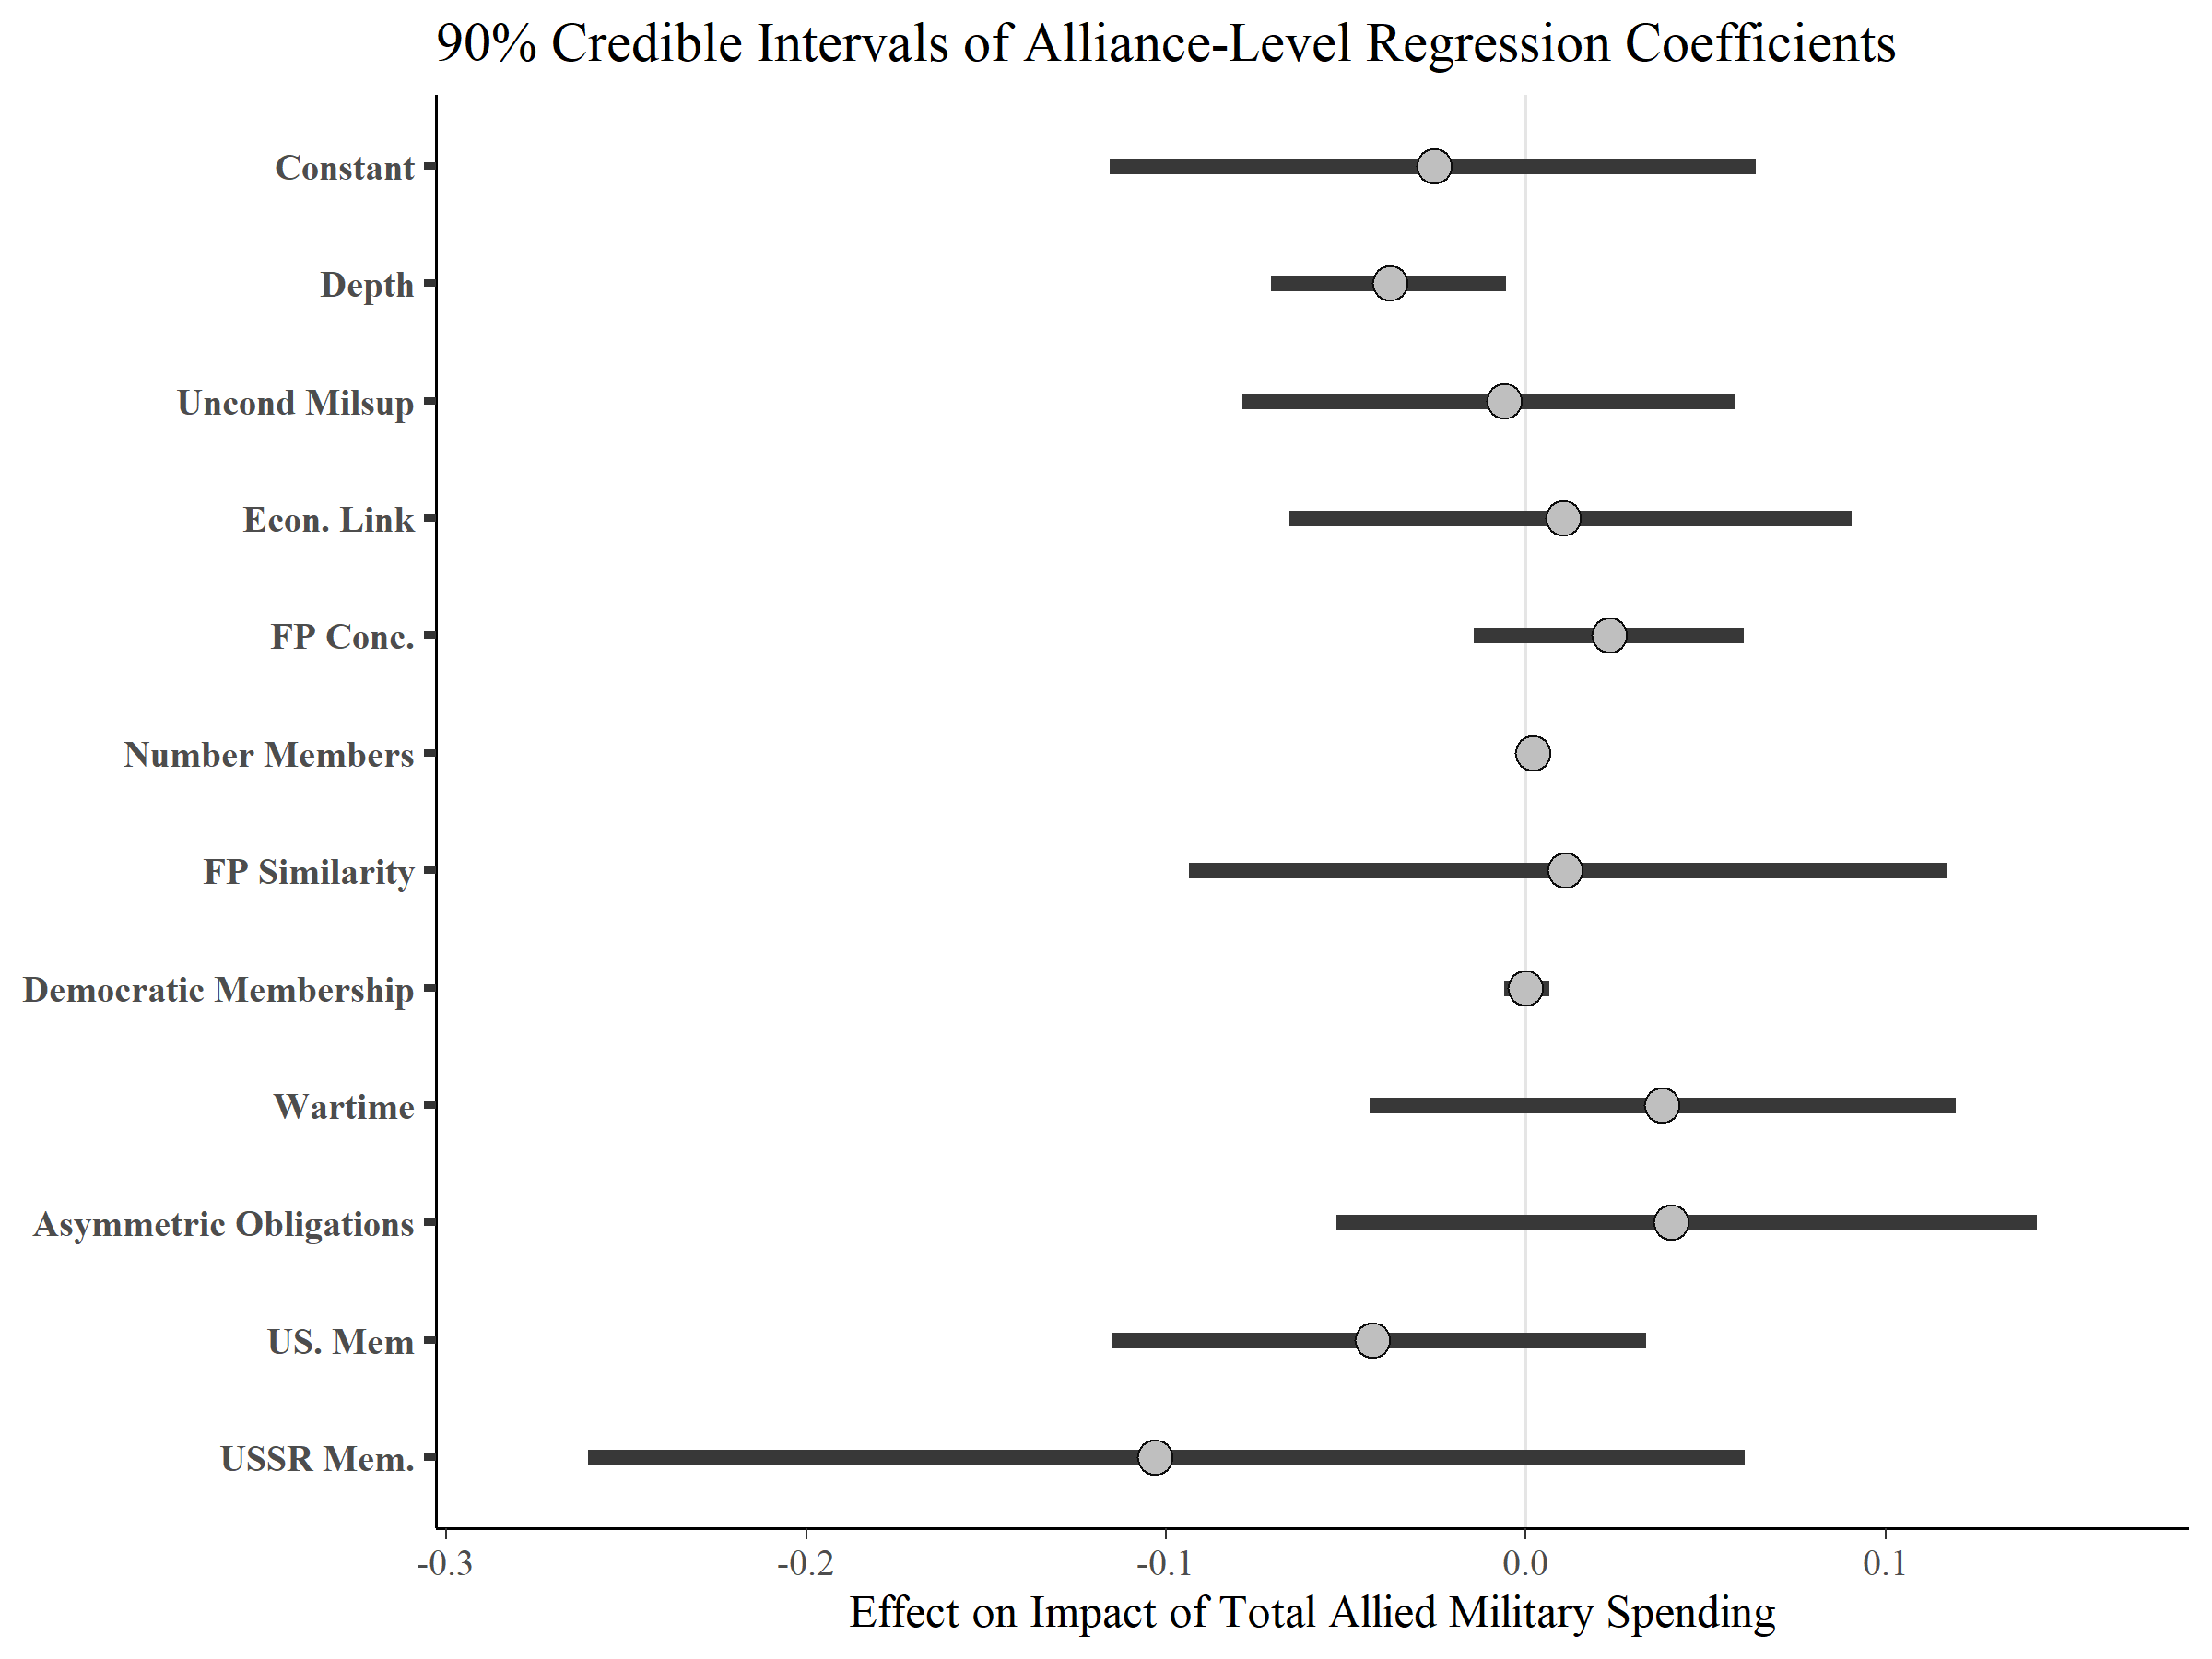
\includegraphics[width=0.95\textwidth]{../figures/alliance-reg-nonmaj.png}
	\caption{90\% credible intervals to summarize the posterior densities of coefficients in the alliance-level regression. Points mark the posterior mean, and the bars encapsulate the width of the credible interval.}
	\label{fig:alliance-reg-nonmaj}
\end{figure}


The preponderance of evidence matches the predictions of Hypothesis 1. 
There is a 96\% chance treaty depth is negatively associated with percent changes in military spending for non-major powers.
The 90\% credible interval for treaty depth does not include zero, though it is close. 
This is one important indicator that participation in a deep alliance increases non-major power military spending, relative to a shallow alliance. 


Treaty depth also has a substantively important effect, which I assessed by simulating the effect of changing treaty depth from the minimum value of -0.8 to 1, which is in the third quartile. 
Holding other alliance covariates at their means, this change in depth reduces the mean of a hypothetical $\lambda$ by .06.
As a result of this change in $\lambda$, the model predicts that percentage changes in alliance members' military spending would fall by .02, for an alliance with median capability. 
The 90\% credible interval of this predicted difference in military spending due to increasing treaty depth ranges from -0.04 to -0.001. 


The substantive importance of treaty depth is reflected by patterns in the $\lambda$ parameters. 
Each $\lambda$ measures the impact of treaty participation. 
If treaty depth has a large influence on alliance participation, it will appear in the $\lambda$ estimates. 
There should be a negative trend in the expected value of $\lambda$ as treaty depth increases in non-major power alliances.
On average, deep alliances should have a negative effect on members' percent changes in military spending and shallow alliances should have a positive effect.  


\begin{figure}[htbp]
	\centering
		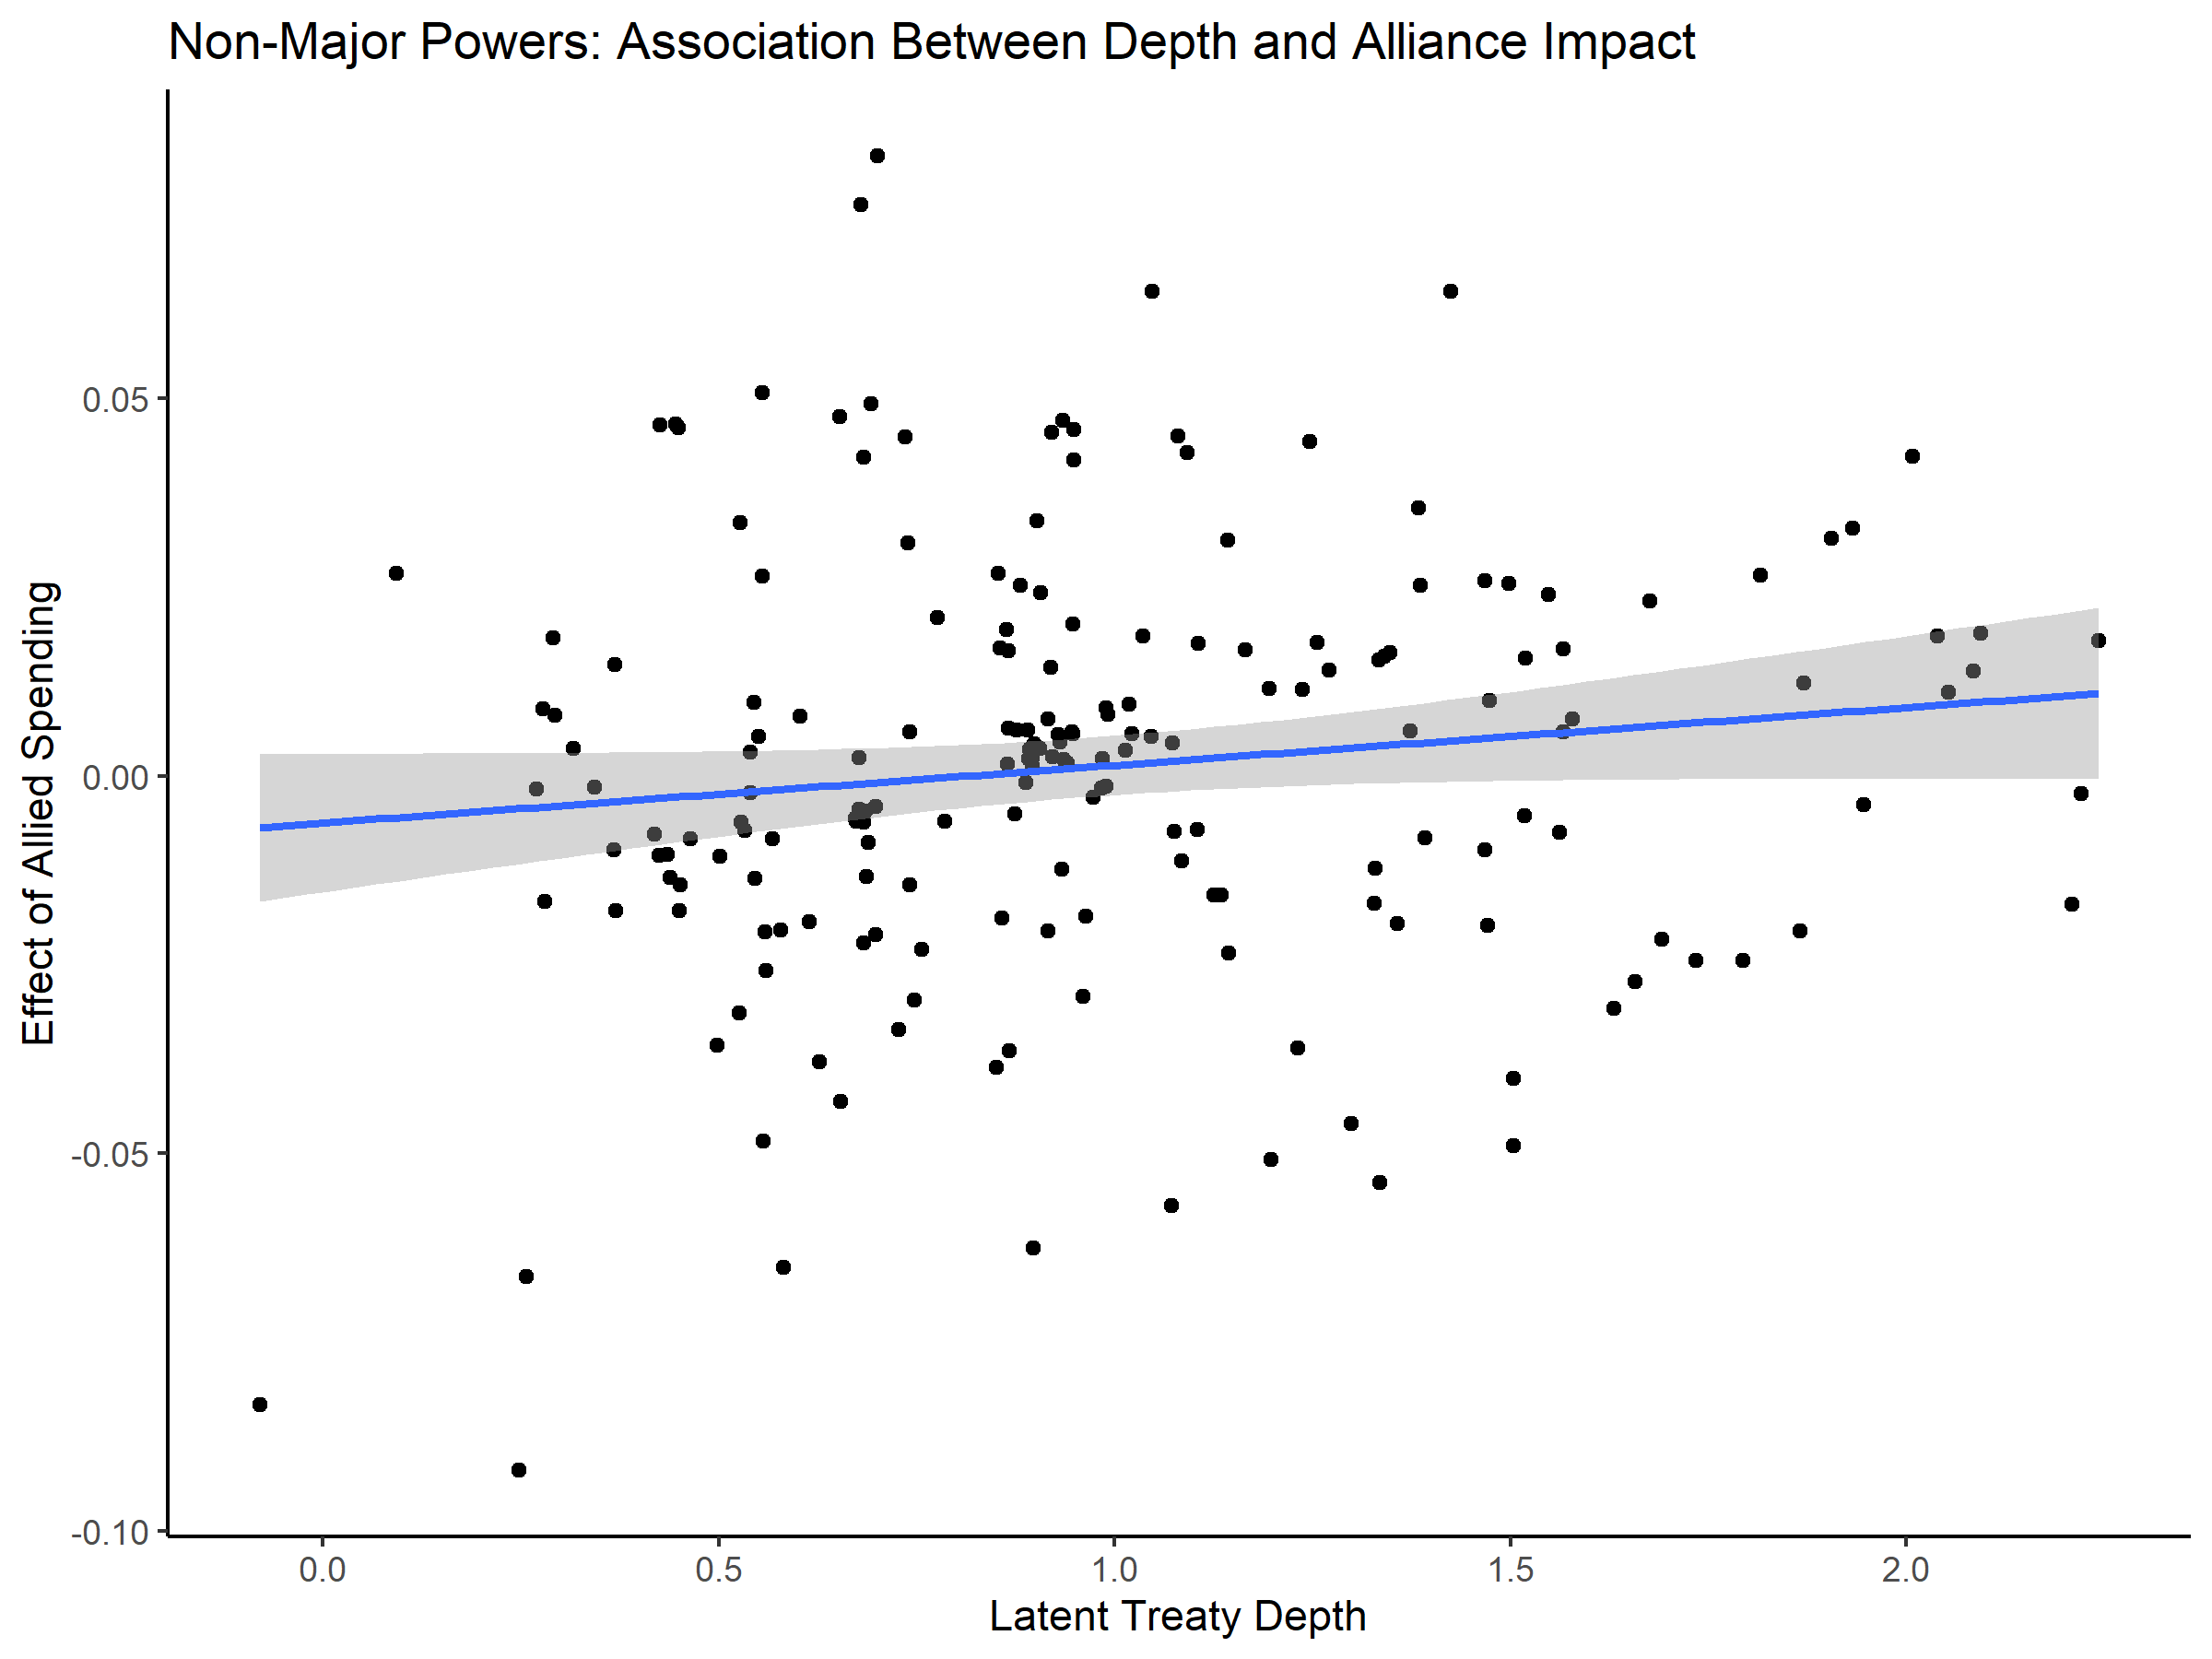
\includegraphics[width=0.95\textwidth]{../figures/lambda-ld-nonmaj.png}
	\caption{Scatter plots of trends in mean $\lambda$ parameters and treaty depth in peacetime alliances. $\lambda$ is the total impact of alliance participation on percent changes in military spending. For non-major powers, $\lambda$ decreases as treaty depth rises. Trend line estimated using linear regression.}
	\label{fig:lambda-ld-nonmaj-peace}
\end{figure}


\autoref{fig:lambda-ld-nonmaj-peace} plots the expected value of $\lambda$ across the range of treaty depth. 
The strong negative correlation between mean $\lambda$ and treaty depth matches the logic of Hypotheses 1. 
Participation in shallow treaties often increases percentage changes in military spending among non-major powers, while most deep treaties have a negative effect. 
Because other treaty characteristics and unmeasured factors also influence the $\lambda$ estimates, \autoref{fig:lambda-ld-nonmaj-peace} shows tremendous variation in how alliance participation impacts non-major power military spending. 


In summary, I find that treaty depth decreases the impact of alliance participation on military spending. 
Deep alliances reduce members military spending, while shallow alliances often increase it. 
This has important consequences for our understanding of alliance participation and military spending. 



\section*{Discussion}


% Precise interpretation: compares alliances. Not treaty vs absence. 
My findings add to our understanding of alliance participation and military spending and address debates over whether alliance participation increases or decreases military spending. 
Claims alliance participation only increases or decreases military spending are incomplete. 
My argument shows how treaty depth modifies the impact of alliance participation on military spending and builds on other conditional arguments \citep{DigiuseppePoast2016}. 


Whether alliance participation increases or decreases military spending depends on treaty depth. 
Compared to no alliance at all, joining a shallow treaty usually increases military expenditures, while participation in a deep alliance often lowers defense spending. 
Greater treaty depth reduces the impact of alliance participation on non-major power military spending. 


How do the findings compare to prior evidence on alliance participation and military spending? 
Connecting my results with earlier evidence requires renewed attention to specific and general research designs. 
General studies compare states in an alliance to those without one. 
Specific studies estimate responsiveness to allied military spending in a few treaties. 


The results encompass specific and general studies, as I estimate both the impact of individual treaties and general differences between treaties. 
My research design emulates specific studies by estimating the unique impact of participation in individual treaties, relative to no alliance. 
The alliance-level coefficients compare treaties to assess the general role of alliance characteristics.   
The specific impact of joining an alliance depends on depth and other alliance characteristics. 


My findings only address formal treaty depth, however. 
The measure of treaty depth only includes formal promises, in part because informal depth is harder to observe. 
As a result, my test of alliance depth may be conservative--- it does not capture phenomena that should have a similar effect. 


% Strategic treaty design
Strategic alliance design is another possible weakness of the test. 
Domestic politics \citep{Davis2004} and democracy \citep{Chibaetal2015} may lead to more arms-length cooperation, for example.   
To address this issue, I controlled for correlates of alliance participation and treaty depth at each level of the model, but selection into different alliances could still produce systematic differences between alliances that are not captured in my statistical model. 


Despite these limitations, the argument and results provide valuable insights about alliance participation and military spending. 
I explain when alliance participation is associated with more or less military spending among non-major powers, addressing debate between contradictory views of alliances.  
I provide evidence that how alliance participation impacts military spending depends on state capability and alliance treaty depth using a new measure of alliance treaty depth and a multilevel model. 
The argument and findings have implications for scholars and policymakers. 


\section*{Conclusion}

% tie it all together
Alliance participation does not uniformly increase or decrease military spending. 
Treaty depth reduces the impact of alliance participation on non-major power defense expenditures. 
As a result, there is a tradeoff between reassurance and free-riding in alliances. 


% Start conclusion
There are several implications of my findings.  
First, they reinforce the importance of accounting for heterogeneity among alliances.
Alliances have heterogeneous effects on the risk of war, trade and military spending \citep{Leeds2003, LongLeeds2006, Benson2012, DigiuseppePoast2016}. 


% Add paragraph on distributional consequences.
The distributional consequences of changes in military spending within states and among alliance members are another implication.  
By altering military spending, alliance design changes the domestic political economy of member states. 
The economic consequences of alliance participation are a possible subject for future research. 


% The argument indicates tradeoff
Besides their scholarly value, the argument and evidence help inform policy debates. 
Tradeoffs in alliance treaty design add to our understanding of why some treaties lead to free-riding and possible policy responses. 
Reassurance from deep alliances increases free-riding. 
States can use deep cooperation to increase alliance credibility, but they lose leverage to check free-riding as a result. 


% Implications for policy. 
The United States is currently wrestling with the implications of treaty depth. 
Washington has often decried free-riding by allies who provide too little for their own defense \citep{Lanoszka2015}. 
But allies are able to free-ride partly because the United States makes deep commitments. 
Attempts to reassure NATO allies may outweigh promises to spend at least 2\% of GDP on defense, for instance.


Reducing the depth of US alliances could generate credibility problems, however. 
Free-riding may be the price of credible commitments.  
Therefore, this paper reveals a tradeoff--- it is not an unconditional call to reduce the depth of US alliances. 
Adjusting existing treaties may be more difficult than designing new alliances and will have other ramifications. 
The full consequences of shifting treaty depth require additional scrutiny. 

 



%\singlespace
 
\bibliography{../../MasterBibliography} 





\end{document}
